\documentclass[a4paper , 12pt]{article}
\usepackage[utf8]{inputenc}
\usepackage{color,soul}
\usepackage[english, francais]{babel}
\usepackage[T1]{fontenc}
\usepackage{graphicx}    % pour inclusion d'image
\usepackage[colorlinks=true]{hyperref}
\usepackage{setspace}
\usepackage{makeidx}
\usepackage{latexsym}
\usepackage{amssymb}
\usepackage{amsmath}
\usepackage{enumitem}
\usepackage{listings}

\usepackage{fancyhdr}
\lhead{Techniques à Objets Avancés}
\rhead{M1 ALMA }
\lfoot{Université de Nantes}
\rfoot{2011-2012 }
\renewcommand{\footrulewidth}{1px}
\pagestyle{fancy}

% \lstset{
% basicstyle=\ttfamily\small, %
% identifierstyle=\color{colIdentifier}, %
% keywordstyle=\color{colKeys}, %
% stringstyle=\color{colString}, %
% commentstyle=\color{colComments}
% language=java

% }*/

\title{\bf Eclipse Vision System Plugin}
\author{Diallo Algassimou}

\begin{document}
\maketitle
\tableofcontents

\part*{Présentation générale}
\section{Introduction}
Eclipse Vision Système permet de détecter des faits à partir d'un flux d'images et de créer des posts sur un réseau social. L'origine du flux d'images, les traitements apportés aux images ainsi que les faits recherchés dans celles-ci et les posts publiés sur un réseau social sont autant de points de variations qui sont pris en compte par Eclipse Vision Système.

\section{Architecture}
Eclipse Vision Système définit deux plugins pour des points d'extensions d'eclipse :
\begin{itemize}
\item actionSets (pour lancer le système) (plugin systemVideo).
\item PreferencePages (Permet d'avoir une page de préférences pour notre système) (plugin PreferencePages).
\end{itemize}

\begin{figure}
  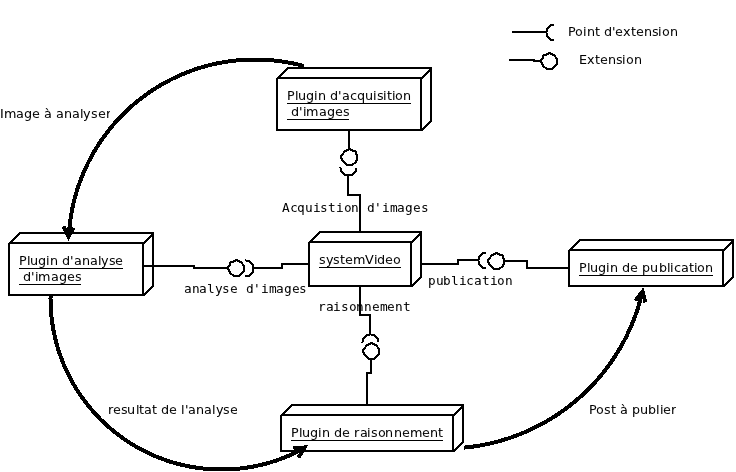
\includegraphics[scale=0.5]{images/architecture.png}
  \caption{Architecture}
  \label{fig:architecture}
\end{figure}

systemVideo est le plugin centrale de notre système. Il fournit quatre points d'extensions qui permettent de capturer toutes les variations possibles dans l'utilisation du système. Ces points d'extensions sont les suivants:
 
\begin{itemize}
\item {\it imageAcquisitionExt} : point d'extension pour les plugins d'acquisition (capture) d'images; 
\item {\it imageAnalysisExt} : point d'extension pour les plugins d'analyse d'images;
\item {\it imageReasonigExt} : point d'extension pour les plugins de traitement d'images ou de raisonnement avant publication; 
\item {\it imagePublicationExt} :point d'extension pour les plugins de publication de posts.
\end{itemize}  
Les plugins suivants ont été développés et peuvent être utilisés : 
\begin{itemize}
\item {\bf imageAcquisitionCamera} : plugin de capture d'une image à partir d'une webcam; 
\item {\bf imageAcquisitionVideo} :  plugin de capture d'une image à partir d'une vidéo;
\item {\bf imageAnalysis} : plugin d'analyse d'une image (reconnaît des visages dans une image); 
\item {\bf imageReasoningSimple} : Publie si l'image contient plus d'un certains nombre de visages ;
\item {\bf imagePublishBlogger} :  publie Un message sur un google blog.
\end{itemize}  

\part*{Installation}
\section{bibliothèque requise}
les bibliothèques suivantes sont requises pour pouvoir faire fonctionner notre système :
\begin{itemize}
\item OpenCV
\item javaCV
\item xuggler
\end{itemize}
Nos plugins ne fonctionne qu'en les lançant avec eclipse.
\part*{Tutoriel}
\section{PagePreference}
\begin{figure}
  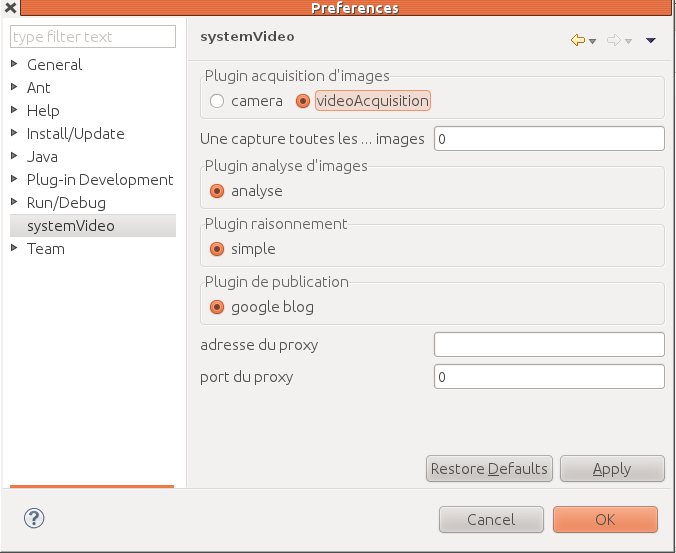
\includegraphics[scale=0.45]{images/preference.png}
  \caption{Page de préférences}
  \label{fig:preferences}
\end{figure}
La page de préférences permet pour chacun des points d'extensions à l'utilisateur de choisir le plugin qu'il veut parmi tous ceux disponibles, et aussi il peut renseigner l'adresse d'un serveur proxy et le port de celui-ci.
On arrive à la page de préférences en cliquant sur : window > Preferences > systemVideo.

\section{exécution}
Dans cette exécution nous allons considérer que les options ont été fixées comme le montre la figure \ref{fig:preferences}.
\subsection{imageAcquisitionVideo}
Ce plugin va capturer les images partir d'une vidéo pour cela il va demander le chemin de la vidéo (figure \ref{fig:fichier_video}).
\begin{figure}
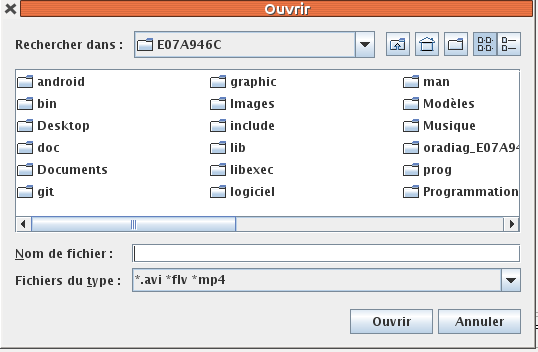
\includegraphics[scale=0.4]{images/fichier_video.png}
\caption{Chemin du fichier vidéo}
\label{fig:fichier_video}
\end{figure}
\subsection{imageAnalysis}
Ce plugin analyse une image à la recherche de visages. Pour cela il a besoin d'un fichier permettant de définir ce qu'est un visage. Ce fichier est fourni par défaut avec les sources de openCV il suffit de renseigner le chemin du fichier (haarcascade\_frontalface\_alt.xml) dans la fenêtre qui s'ouvre (voir figure \ref{fig:haar}).

\begin{figure}
  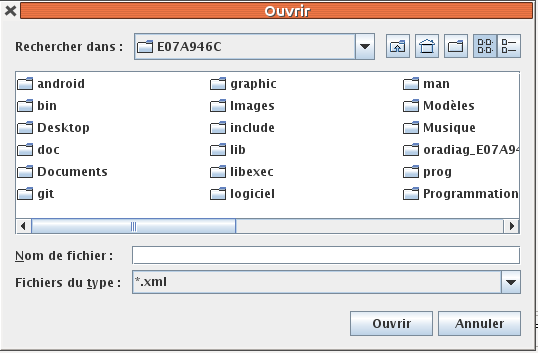
\includegraphics[scale=0.5]{images/figureHaar.png}
  \caption{fichier définissant un visage}
  \label{fig:haar}
\end{figure}

\subsection{imageReasoning}
Ce plugin compte le nombre d'images trouvées par le plugin précèdent et post un billet sur le blog si le nombre de visage dépasse un certains nombre (Ce nombre est renseigné par l'utilisateur comme le montre la figure \ref{fig:nombre_visages}).

\begin{figure}
  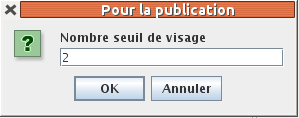
\includegraphics[scale=0.5]{images/nombre_visages.png}
  \caption{Le nombre seuil de visages}
  \label{fig:haar}
\end{figure}

\subsection{imagePublishBlogger}
Ce plugin permet la publication de post sur un blog google. Pour cela il demande en paramètres les identifiant de connexion ainsi le nom de l'auteur du post (voir figure \ref{fig:google}).

\begin{figure}
  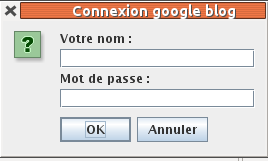
\includegraphics[scale=0.45]{images/google.png}
  \caption{identifiant de connexion compte google}
  \label{fig:google}
\end{figure}

\part*{Utilisation avancée}
Comme le montre la figure \ref{fig:architecture} systemVide définit quatre points d'extensions. Pour écrire un plugin pour systemVideo on choisit l'un de ces points d'extensions et on définit une classe qui implémente l'interface du point d'extension.

Notre système est un chaînage de plugin car le plugin d'acquisition d'image capture une image et la passe au plugin d'analyse qui lui analyse l'image et passe ces résultats au plugin de raisonnement qui traite les résultats et décide de publier ou non.

  \section{Points d'extension et interfaces} 
  \subsection{acquisition d'image}
  L'interface de ce point d'extension est la suivante :
  \lstinputlisting{interfaces/IImageAcquisition.java}
  \subsubsection*{méthode run}
  Cette méthode est appelé par le plugin centrale (systemVideo). elle lance réellement l'exécution du système.
  \subsubsection*{méthode init}
  Cette méthode est appelé pour initialiser le plugin. Elle est appelé avant la méthode run et peut être utilisé pour demander des informations à l'utilisateur (chemin d'un fichier , un identifiant etc).
  \subsubsection*{méthode setIImageAnalysis}
  Cette méthode permet de fixer le l'objet qui va analyser les images capturées.
  \subsection{analyse d'image}
 \lstinputlisting{interfaces/IImageAnalysis.java}
  \subsubsection*{méthode analyse}
  Cette méthode est appelé par le plugin d'acquisition d'image et à comme paramètre l'image capturer.
  \subsubsection*{méthode init}
  Cette méthode est appelé une seule fois (avant toute autres méthodes) et peut permettre au plugin de s'iniatialiser.
  \subsubsection*{méthode setIImageResoning}
  Cette méthode permet de fixer le l'objet qui va recevoir les résultats de nos analyse.

  \subsection{raisonnement}
 \lstinputlisting{interfaces/IImageReasoning.java}
  \subsubsection*{méthode reasoning}
  Cette méthode est appelé par le plugin d'analyse d'image et à comme paramètre une liste d'objets issue de l'analyse.
  On peut remarquer que cette liste peut être une liste de n'importe qu'elle objet java, ainsi pour pouvoir raisonner au mieu ce plugins doit connaître qu'elle sont les type concrets de objets envoyer et dans qu'elle ordre ce qui crée une forte dépendances entre le plugin d'analyse et le plugin de raisonnement.
  \subsubsection*{méthode init}
  Cette méthode est appelé une seule fois (avant toute autres méthodes) et peut permettre au plugin de s'iniatialiser.
  \subsubsection*{méthode addIImagePublish}
  Cette méthode permet d'ajouter un IImagePublis (un plugin pour la publication de post  ceux connu du plugin de raisonnent). Ainsi un même peut être publier sur différents réseaux sociaux.

  \subsection{publication de post}
  \lstinputlisting{interfaces/IImagePublish.java}
  \subsubsection*{méthode publish}
  Cette méthode est appelé par le plugin de raisonnement. Elle prend en paramètre l'image à publier, le titre du post et le contenu du post.
  \subsubsection*{méthode init}
  Cette méthode est appelé une seule fois (avant toute autres méthodes) et peut permettre au plugin de s'iniatialiser.
  \subsubsection*{méthode setProxyHost}
  Cette méthode permet de prendre en compte l'adresse du proxy. Elle est appelé une seule fois et avant la méthode publish
  \subsubsection*{méthode setProxyPort}
  Cette méthode permet de prendre en compte le port du proxy. Elle est appelé une seule fois et avant la méthode publish
\end{document}
